\documentclass[tikz, border=10pt]{standalone}
\usepackage{pgfplots}
\usepackage{amsmath}
\usetikzlibrary{backgrounds}
\pgfplotsset{compat=1.18}

\begin{document}
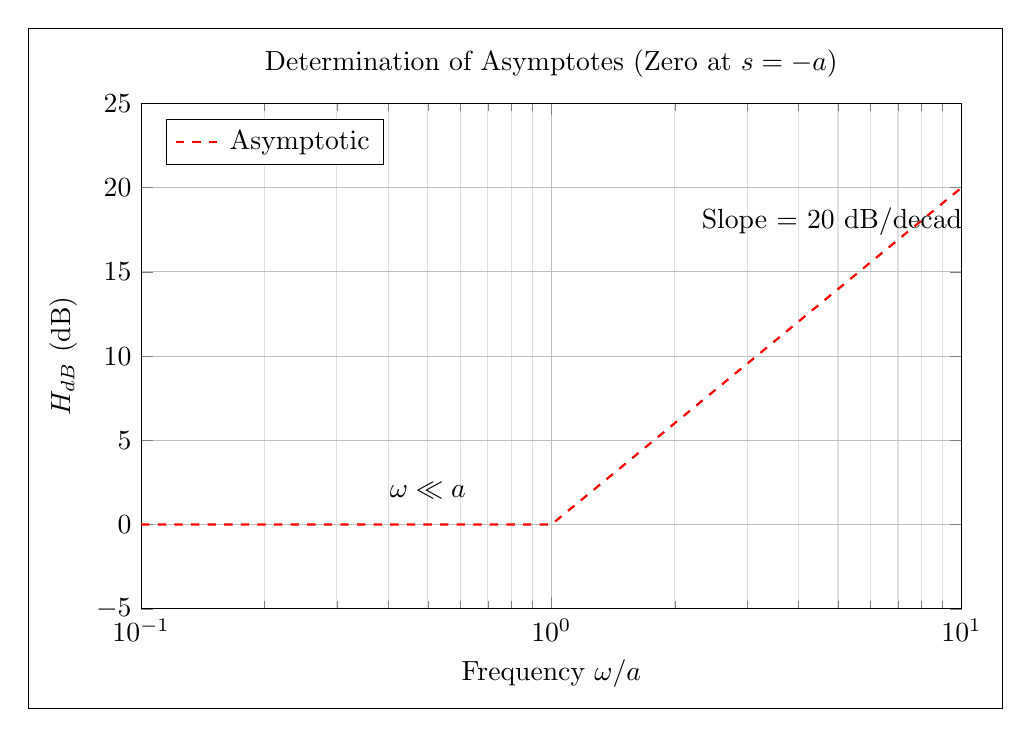
\begin{tikzpicture}[show background rectangle]
    \begin{semilogxaxis}[
        width=12cm, height=8cm,
        title={Determination of Asymptotes (Zero at $s = -a$)},
        xlabel={Frequency $\omega/a$},
        ylabel={$H_{dB}$ (dB)},
        grid=both,
        xmin=0.1, xmax=10,
        ymin=-5, ymax=25,
        minor grid style={gray!25},
        major grid style={gray!50},
        legend pos=north west,
    ]

    % Asymptote: 0 for w < a, 20log(w/a) for w > a
    % using coordinates for the corners
    \addplot[red, dashed, thick, domain=0.1:10] coordinates {
        (0.1, 0) (1, 0) (10, 20)
    };
    \addlegendentry{Asymptotic}

    % Legend and labels handled by pgfplots
    \node at (axis cs:0.5, 2) {$\omega \ll a$};
    \node at (axis cs:5, 18) {Slope = 20 dB/decade};
    
    \end{semilogxaxis}
\end{tikzpicture}
\end{document}
